\section{项目详细设计}
\begin{frame}
    \frametitle{核心算法设计}
    \footnotesize
    \begin{itemize}
        \item {词法分析器:基本架构采用一个DFA,由nextChar()获取的下一个字符标识DFA状态,数据粒度为字符,对外的接口是run和nextToken(一遍过程中由Parser调用)}
        \item {语法分析器:两套语法分析器分别采用LR(1)分析方法和递归下降语法分析方法。在实际开发中,随着我期望实现的语言特性越来越多,LR(1)方法中的文法设计变得愈发困难,因此该方法实现的语法分析器在项目后期我已经停止维护,而使用递归下降的方法实现了所有下述的编译器功能特性。}
        \item {中间代码生成器:实际开发中采用访问者模式实现,同样使用两套生成器,采用语法制导的翻译方法。对于代码中每个文法节点的gen方法传入不同的目标代码生成器对象指针,就能够生成不同表示形式的中间代码。}
        \item {目标代码生成器:通过LLVM Target中提供的相关接口,直接将LLVM IR形式的中间代码映射到对应target下的目标代码,并且使用LLVM Pass实现不同等级的代码优化逻辑。}
        \item {可执行文件生成:依赖第三方编译环境提供的类库实现和链接器}
    \end{itemize}
\end{frame}

\begin{frame}
    \frametitle{类设计}
    \footnotesize
    \begin{itemize}
        \item {File类:用于储存读入的源文件内容,提供了操作文件的相关接口,包括数据获取、移动行号、信息记录等等}
        \item {Lexer类:词法分析器实现主体类,在一遍过程中为语法分析器提供nextToken()接口用于推进分析过程}
        \item {Parser和LR1Parser类:实现了递归下降和LR1分析两种语法分析方法的语法分析器实现主体类,输出相同的AST数据结构}
        \item {LLVMIRGenerator和IRGenerator类:分别使用语法制导翻译技术,输出LLVM IR和四元式形式表示的中间代码序列}
        \item {CodeGenerator类:使用LLVM IR中间代码序列作为输入,执行代码优化逻辑后输出可执行的目标文件}
        \item {相关工具类:包括错误处理、日志记录、运行时参数解析等于项目实现相关的工具类,可在源码中查看,此处不再赘述}
        \item {AST节点类:本实验中的AST节点类设计参考了Clang源码中的设计架构,为每种实现需求中的文法符号实现了对应的节点类型定义,此处重点阐述其中所有类型的具体含义}
    \end{itemize}
\end{frame}

\begin{frame}
    \frametitle{AST节点类型设计}
    \footnotesize
    {本实验中的AST节点类型根据C语言文法符号设计进行定义,以ASTNode节点作为类型继承树根,主要分为三大子类型,其中子类型进一步衍生出其它的文法符号定义类型}
    \begin{itemize}
        \item {lcc::AST::Decl(Declaration):声明类型,包括变量声明、函数声明、结构体声明、枚举声明等等}
        \item {lcc::AST::Stmt(Statement):语句类型,包括赋值语句、函数调用语句、控制流语句、循环语句等等}
        \item {lcc::AST::Expr(Expression):表达式类型,包括常量表达式、变量表达式、函数调用表达式、运算表达式等等}
    \end{itemize}
\end{frame}

\begin{frame}
    \frametitle{AST节点类型设计}
    \footnotesize
    \begin{itemize}
        \item {lcc::AST::ASTNode:该类型是所有抽象语法树节点类型的基类(抽象类),作为一个接口类,声明了所有AST节点类型必须实现的asJson和gen方法}
        \item {lcc::AST::Decl:所有声明性质节点的基类(抽象类)}
        \item {lcc::AST::TranslationUnitDecl:该类型是AST的根节点类型,表示顶层的声明上下文,该节点的孩子是若干个顶层Decl节点}
        \item {lcc::AST::NamedDecl:该抽象语法树节点表示可能具有名字的声明(或者定义)类型,本项目中的FunctionDecl、VarDecl以及其它具有名字的声明对应的AST节点类型均为该类型的派生类}
        \item {lcc::AST::VarDecl:该抽象语法树节点表示变量的声明(或者定义),即类似int a;的声明语句或者int a = 1 + 2;的定义语句}
        \item {lcc::AST::ParmVarDecl:该抽象语法树节点表示函数声明或者定义圆括号(paren)之间的形参,即类似... ...(int a, int b)中的int a, int b}
        \item {lcc::AST::FunctionDecl:该抽象语法树节点表示函数的声明(或者定义),即类似int func(int param);的声明语句或者int func(int param){ ... }这样的定义语句}
    \end{itemize}
\end{frame}

\begin{frame}
    \frametitle{AST节点类型设计}
    \footnotesize
    \begin{itemize}
        \item {lcc::AST::Expr:所有表达式性质节点的基类(抽象类)}
        \item {lcc::AST::BinaryOperator:该抽象语法树节点类型表示一个双目运算符表达式,维护表达式的左部,符号和右部信息(例如a+b)}
        \item {lcc::AST::UnaryOperator:该抽象语法树节点类型表示一个单目运算符表达式,维护表达式的符号和右部信息(例如!a)}
        \item {lcc::AST::CastExpr:该抽象语法树节点类型表示一个类型转换表达式,所有类型转换表达式类型的基类}
        \item {lcc::AST::ImplicitCastExpr:该抽象语法树节点类型表示一个隐式类型转换表达式}
        \item {lcc::AST::DeclRefExpr:该抽象语法树节点类型表示一个对变量或者函数的引用}
        \item {lcc::AST::CallExpr:该抽象语法树节点类型表示一个函数调用表达式,即形如func(1,2)之类的式子}
        \item {lcc::AST::ParenExpr:该抽象语法树节点类型表示一个括号表达式,其基本形式为( Expr ),即前缀和后缀分别为左右括号(Expr),中间包裹一个表达式。}
    \end{itemize}
\end{frame}

\begin{frame}
    \frametitle{AST节点类型设计}
    \footnotesize
    \begin{itemize}
        \item {lcc::AST::IntegerLiteral:该抽象语法树节点类型表示一个整形数字面量,即数值1,-2,321等等类似的整形数}
        \item {lcc::AST::FloatingLiteral:该抽象语法树节点类型表示一个浮点数字面量,支持下列6种浮点数表示法}
    \end{itemize}
\end{frame}

\begin{frame}
    \frametitle{AST节点类型设计}
    \footnotesize
    \begin{itemize}
        \item {lcc::AST::Stmt:该抽象语法树节点类型表示一个语句,Clang中对于该类型的描述如下}
        \item {lcc::AST::CompoundStmt:该抽象语法树节点类型表示一个混合语句。所谓混合语句,就是以大括号围起来的若干语句集合}
        \item {lcc::AST::WhileStmt:该抽象语法树节点类型表示一个While循环语句,即类似while(1){ ... }的语句}
        \item {lcc::AST::IfStmt:该抽象语法树节点类型表示一个if条件分支语句,包括if和if...else...两大类。}
        \item {lcc::AST::ReturnStmt:该抽象语法树节点类型表示一个返回语句,包括返回一个值(即表达式)或者返回空两种情况}
        \item {lcc::AST::NullStmt:该抽象语法树节点类型表示一个空语句}
        \item {lcc::AST::DeclStmt:该抽象语法树节点类型表示一个变量声明或者定义语句}
        \item {lcc::AST::ValueStmt:该抽象语法树节点类型表示数值语句,即一个表达式(Expr)}
        \item {lcc::AST::AsmStmt:该抽象语法树节点类型表示一个GCC风格内联汇编语句,语法规范如下图所示}
    \end{itemize}
\end{frame}

\begin{frame}
    \frametitle{AST节点类型设计}
    \footnotesize
    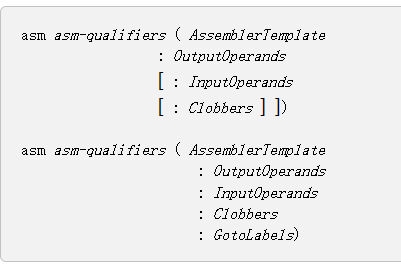
\includegraphics[width=\textwidth]{contents/figure/asm.png}
\end{frame}

\begin{frame}
    \frametitle{AST节点类型设计}
    \footnotesize
    \begin{itemize}
        \item {lcc::AST::ArraySubscriptExpr:该抽象语法树节点类型表示一个数组索引语句(比如a[0], arr[idx]等等)}
    \end{itemize}
\end{frame}
